\documentclass{article}
\usepackage[utf8]{inputenc}

\title{MATH2710 — Portfolio 4.1 - 7.1}
\author{Mike Medved}
\date{March 23rd, 2023}

\usepackage{color}
\usepackage{amsthm}
\usepackage{amssymb} 
\usepackage{amsmath}
\usepackage{lmodern}
\usepackage{mathtools, nccmath}
\usepackage{listings}
\usepackage[margin=1in]{geometry} 
\usepackage[table,xdraw,dvipsnames]{xcolor}
\usepackage{tikz}
\usepackage{pgfplots}

\usepackage{xparse}
%
\DeclarePairedDelimiterX{\set}[1]{\{}{\}}{\setargs{#1}}
\NewDocumentCommand{\setargs}{>{\SplitArgument{1}{;}}m}
{\setargsaux#1}
\NewDocumentCommand{\setargsaux}{mm}
{\IfNoValueTF{#2}{#1} {#1\,\delimsize|\,\mathopen{}#2}}%{#1\:;\:#2}

\parindent = 0pt

\newtheorem*{thm}{Theorem}

\begin{document}

\maketitle

\section*{Mathematical Components}

\subsection*{Lemma}

\textbf{Definition:} A true and simple mathematical statement whose main purpose is to help a theorem.

\textbf{Example:} \textit{If $x$ is a real number, then $x^2$ is a real number.}

\subsection*{Theorem}

\textbf{Definition:} A true mathematical statement of significant importance that has been proved to be true.

\textbf{Example:} The Pythagorean Theorem is famous example of a theorem, it is shown below.


\begin{center}
    % use tikz to make a right triangle with sides labelled a, b, c
    \begin{tikzpicture}[scale=1.5]
        \draw (0,0) -- (2,0) -- (2,1) -- cycle;
        \draw (0,0) -- (2,1);
        \draw (0,0) node[below] {$a$};
        \draw (2,0) node[right] {$b$};
        \draw (2,1) node[above] {$c$};
    \end{tikzpicture}
\end{center}

\begin{equation*}
a^2 + b^2 = c^2
\end{equation*}

\subsection*{Corollary}

\textbf{Definition:} A true mathematical statement that is an immediate consequence of a theorem or proposition.

\textbf{Example:} Take the below theorem as an example. Below, you will see a corollary that is an immediate consequence of the theorem.

\begin{thm}
    If $\displaystyle\lim_{x \to \infty} f(x) = \ell$, then $\forall (a_n) m \geq 1, a_n \xrightarrow{n \to \infty} \infty, f(a_n) \xrightarrow{n \to \infty} \ell$.
\end{thm}

\begin{center}
    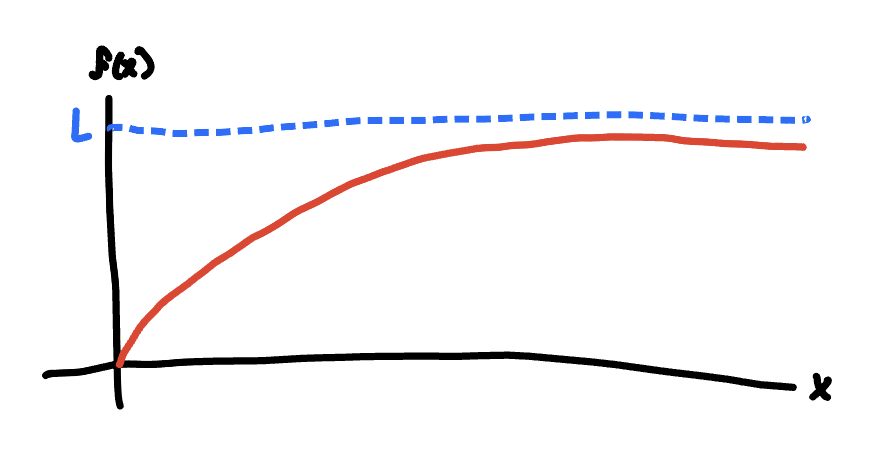
\includegraphics[scale=0.25]{corollary-example.jpeg}
\end{center}

\newpage
\textbf{Corollary.} $\displaystyle\lim_{x \to \infty} sin(x)$ DNE.

\begin{center}
    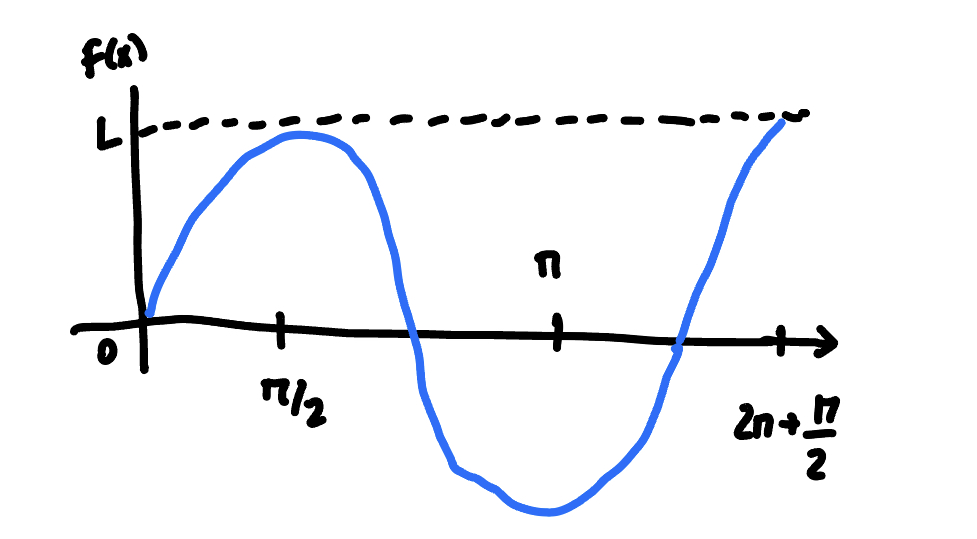
\includegraphics[scale=0.25]{corollary-example2.jpeg}
\end{center}

\begin{proof}
    We aim to prove the above corollary.
    $\hfill \break$
    $\hfill \break$
    For $a_n = 2n\pi + \frac{\pi}{2} \rightarrow \infty$, we have $f(a_n) = 1 \xrightarrow{n \to \infty} 1$ \\
    For $b_n = 2n\pi - \frac{\pi}{2} \rightarrow \infty$, we have $f(a_n) = -1 \xrightarrow{n \to \infty} -1$ \\

    $\xRightarrow{Theorem \text{ 1 }} sin(x)$ does not have a limit as $x \to \infty$.
\end{proof}

\section*{Direct Proof}

\subsection*{Outline}

A direct proof for a statement $P \Rightarrow Q$ takes the following form:

\begin{enumerate}
    \item Assume $P$ is true, to prove: $Q$.
    \item To prove: $Q_1$.
    \item $...$
    \item To prove $Q_n$.
\end{enumerate}

In this way, $Q$ will be transformed from $Q_1 \to Q_n$ through a series of logical implications.

\subsection*{Examples}

\subsubsection*{Divisibility of Three Integers}

Let $(a, b, c) \in \mathbb{Z}$, prove that if $a | b$ and $b | c$, then $a | c$.

$\hfill \break$
\textbf{Reminder:} $a | b$ refers to the fact that $\exists n \in \mathbb{Z}, a \cdot n = b$.

\begin{proof}
    We aim to prove that $a$ divides $c$, thus: $\exists n \in \mathbb{Z}, a \cdot n = c$.
    
    \begin{enumerate}
        \item As $a | b$, we have $\exists p \in \mathbb{Z}, a \cdot p = b$
        \item As $b | c$, we have $\exists m \in \mathbb{Z}, b \cdot m = c$
    \end{enumerate}

    From (1) and (2) we get the following: $\exists p, m \in \mathbb{Z}, (a \cdot p) \cdot m = c$. As we already know that $a \cdot p = b$, we may rewrite the above with $a \cdot p = n \in \mathbb{Z}$.

    $\hfill \break$
    Thus, we have found that $\exists n \in \mathbb{Z}, a \cdot n = c.$
\end{proof}

\subsubsection*{Union of Two Bounded Sets}

Let $A, B \subseteq \mathbb{R}$ be bounded sets, prove that $A \cup B$ is bounded.

\begin{proof}
    As $A, B$ are bounded, let's assume that $\exists m, \forall a \in A, m > a$. Similarly, let's assume that $\exists n, \forall b \in B, n > b$. From this, we can say that $k = \text{max}(m, n)$, which means $\forall (a, b), k > a, k > b$. This means $k$ upper-bounds both $A$ and $B$.
    
    $\hfill \break$
    As $k$ upper-bounds both $A$ and $B$, we can say that $A \cup B$ is bounded.
\end{proof}

\section*{Proof by Contrapositive}

\subsection*{Outline}

A proof by contrapositive of a statement $P \Rightarrow Q$ is the direct proof of $\lnot Q \Rightarrow \lnot P$. Thus, the proof by contrapositive takes the following form:

\begin{enumerate}
    \item Assume $\lnot Q$ is true, to prove: $\lnot P$.
    \item Translate $(\lnot P)_1 \to (\lnot P)_n$.
    \item Assume $\lnot Q$, using logical implications show $(\lnot P)_n$ is true.
\end{enumerate}

\subsection*{Examples}

\subsubsection*{Perfect Squares}

Let $n \in \mathbb{N}$, prove that if $n$ is $M_4+2$ or $n$ is $M_4+3$, then $n$ is not a perfect square.

$\hfill \break$
\textbf{Definition 1.} A perfect square $k$ is an integer $k$ such that $\exists n \in \mathbb{N}, n^2 = k$.
$\hfill \break$
\textbf{Definition 2.} $a | b$ is equivalent to $\exists q \in \mathbb{Z}, b = aq$

\begin{proof}
    Assume $n$ is a perfect square, to prove: $n$ is not $M_4+2$ and $n$ is not $M_4+3$.
     
    \begin{enumerate}
        \item \textbf{Case.} $n$ is a $M_{4}+2$
    
        Then, $n = 4k+2$ for some integer $k$. We can rewrite $n$ as $n = 2(2k+1)$.
        
        Notice that $2k+1$ is an odd integer. We know that the square of an odd integer is always odd, so let $2k+1 = 2m+1$ for some integer $m$. Then, $n = 2(2m+1)$.
        
        We can see that $n$ has a factor of $2$ raised to the power of $1$, but no other factors of $2$ in its prime factorization. Therefore, $n$ cannot be a perfect square.

        \item \textbf{Case.} $n$ is a $M_4+3$

        Then, $n = 4k+3$ for some integer $k$. We can rewrite $n$ as $n = 1 + 4k+2$.
    
        Using the same logic as in Case 1, we can see that $n$ has a factor of $2$ raised to the power of $1$, but no other factors of $2$ in its prime factorization. Therefore, $n$ cannot be a perfect square.
        
        Therefore, if $n$ is a $M_{4}+2$ or $M_{4}+3$, then $n$ is not a perfect square.
    
    \end{enumerate}
\end{proof}
\subsubsection*{Divisibility of Two Integers}

Let $x, y \in \mathbb{Z}$, prove that if $\lnot (xy | 11)$, then $\lnot (x | 11)$ and $\lnot (y | 11)$.

\begin{proof}
    Assume $xy | 11$, to prove: $x | 11$ or $y | 11$.
    \begin{enumerate}
        \item \textbf{Case.} If $x = 11c, c \in \mathbb{Z}$, then $xy = 11cy$, thus $xy | 11$.
        \item \textbf{Case.} If $y = 11d, d \in \mathbb{Z}$, then $xy = 11xd$, thus $xy | 11$.
    \end{enumerate}
\end{proof}

\section*{Clarity}

\section*{Proof by Contradiction}

\subsection*{Contradiction of $P$}

A proof by contradiction on a statement of type $P$ is the direct proof of $\lnot P \Rightarrow c$ for some initially unknown contradiction $c$. Thus, the proof by contradiction on $P$ takes the following form:

\begin{enumerate}
    \item To prove: $P$.
    \item To prove: $\lnot P \Rightarrow c$.
    \item Assume $\lnot P$, translate $(\lnot P)_1 \to (\lnot P)_n$ until you arrive at $c$.
\end{enumerate}

\subsection*{Examples}

\subsubsection*{Irrationality of $\sqrt{5}$}

\begin{proof}
    Assume absurdly that $\sqrt{5}$ is rational. $q \in \mathbb{Q}$ take the form $\frac{a}{b}, (a, b) \in \mathbb{Z}, b \neq 0$. Thus, $\sqrt{5} = \frac{a}{b}$ for some $a, b \in \mathbb{Z}, b \neq 0$. We can then square both sides, giving us: $\frac{a^2}{b^2} = 5$. Further, we are able to multiply both sides by $y^2$ to isolate $x^2$, $5y^2 = x^2$.

    $\hfill \break$
    Since $5y^2 = x^2$, they must have the same number of prime factors. This shows that both $x^2, y^2$ have an even number of prime factors, and $5y^2$ has an odd number of prime factors. This is a contradiction, as $5y^2 = x^2$, yet they have a different amount of prime factors. Thus, our assumption was invalidated, and $\sqrt{5}$ is irrational.
\end{proof}

\subsubsection*{Finding $x, y \in \mathbb{Z}$ for $x^2+3y^2=n$}

Let $n$ be an even integer that is not $M_4$, prove by contradiction that we cannot find $x, y \in \mathbb{Z}$ such that $x^2+3y^2=n$.

\begin{proof}
    Assume absurdly that for some $n \in \mathbb{Z}, n \in M_4$, $\exists (x, y) \in \mathbb{Z}, x^2+3y^2=n$. Since $n$ is $M_4$, we can write $n = 4k$ for some $k \in \mathbb{Z}$. Thus, $x^2+3y^2 = 4k$, and $x^2+3y^2 = 4k+1$, and $x^2+3y^2 = 4k+2$, and $x^2+3y^2 = 4k+3$. Thus, $x^2+3y^2$ is congruent to $0, 1, 2, 3$ modulo $4$. This is a contradiction, as $x^2+3y^2$ is congruent to $0, 1, 2, 3$ modulo $4$, yet $n$ is $M_4$. Thus, our assumption was invalidated, and we cannot find $x, y \in \mathbb{Z}$ such that $x^2+3y^2=n$.
\end{proof}

\subsection*{Contradiction of $P \Rightarrow Q$}

A proof by contradiction on a statement of type $P \Rightarrow Q$ is the direct proof of $\lnot (P \Rightarrow Q) \Rightarrow c$ for some initially unknown contradiction $c$. Thus, the proof by contradiction on $P \Rightarrow Q$ takes the following form:

\begin{enumerate}
    \item To prove: $P \Rightarrow Q$.
    \item To prove: $\lnot (P \Rightarrow Q) \Rightarrow c$.
    \item To prove: $(P \land (\lnot Q)) \Rightarrow c$.
    \item Assume $P \land (\lnot Q)$, translate through logical implications until $c$ is discovered.
\end{enumerate}

\subsection*{Similarities with Proof by Contrapositive}

One similarity between the Proof by Contradiction of $P \Rightarrow Q$ and that of the Proof by Contrapositive is that we assume $\lnot Q$ in both proofs.

\subsection*{Differences with Proof by Contrapositive}

One difference between the Proof by Contradiction of $P \Rightarrow Q$ and that of the Proof by Contrapositive is that prove $\lnot P$ in the contrapositive proof, whereas in the contradiction proof we prove a contradiction $c$.

\section*{Biconditionality}

\subsection*{Ways to Read}

\begin{enumerate}
    \item $P \Leftrightarrow Q$ can be read as "$P$ if and only if $Q$".
    \item $P \Leftrightarrow Q$ can be read as "$P$ is a necessary and sufficient condition for $Q$".
    \item $P \Leftrightarrow Q$ can be read as "$P$ is equivalent to $Q$".
\end{enumerate}

\subsection*{Outline}

Use any means necessary to prove the below statements.

\begin{enumerate}
    \item To prove: $P \Rightarrow Q$.
    \item To prove: $Q \Rightarrow P$.
\end{enumerate}

\subsection*{Example 1}

Let $x, y \in \mathbb{Z}$, prove that $4 | x^2-y^2$ iff $x, y$ have the same parity.

\begin{proof}
    First, we must prove $P \Rightarrow Q$. That is, that assuming $4 | x^2-y^2$, we can conclude that $x, y$ have the same parity. 
    
    $\hfill \break$
    Assume $4 | x^2-y^2$, then $x^2-y^2 = 4k$ for some $k \in \mathbb{Z}$. Thus, $x^2 = 4k+y^2$ or $y^2 = 4k+x^2$. Since $x^2, y^2$ are both even, they must both be congruent to $0$ modulo $4$. Thus, $x^2 = 4k+y^2$ or $y^2 = 4k+x^2$ implies that $x^2, y^2$ are both congruent to $0$ modulo $4$. Thus, $x, y$ have the same parity.

    $\hfill \break$
    Now, we must prove the converse, that $Q \Rightarrow P$. That is, that assuming $x, y$ have the same parity, we can conclude that $4 | x^2-y^2$.

    $\hfill \break$
    Assume $x, y$ have the same parity. Since $x, y$ have the same parity, they must both be even or both be odd. Thus, $x^2, y^2$ are both even or both odd. Since $x^2, y^2$ are both even or both odd, they must both be congruent to $0$ modulo $4$. Thus, $x^2 = 4k+y^2$ or $y^2 = 4k+x^2$ implies that $x^2, y^2$ are both congruent to $0$ modulo $4$. Thus, $x^2-y^2 = 4k$ for some $k \in \mathbb{Z}$, and $4 | x^2-y^2$.
\end{proof}

\subsection*{Example 2}

Let $x, y \in \mathbb{Z}$, prove that $x^2=y^2$ iff $x=y$ or $x=-y$.

\begin{proof}
    In the case of this proof, we are able to immediately show that the inequality holds for both $x=y$ and $x=-y$ since $|x|=|y| \Leftrightarrow x = \pm y$. Thus, we do not need to evaluate both $P \Rightarrow Q$ and $Q \Rightarrow P$ explicitly.
\end{proof}

\end{document}